\chapter{Introduction}
\section{Motivation}
Modern large scale spectroscopic surveys generate hundreds of thousands or even millions of spectra. The analysis of these high volume data-sets presents a significant challenge to the researcher as well as to compute infrastructure and engineering. Additionally, if the data is collected by a high resolution instrument, the researcher will face the challenge of wrangling and analysing individual data points with dimensions at the scale of several thousands per spectrum \cite{buder2021galah+}. When the number of data points are of the order of hundreds of thousands (or millions) and when each data point has a dimensionality of several thousands, it becomes impractical and perhaps even infeasible to process and analyse this data using manual methods such as naked eye observations of spectral plots. 

Unless the science goals have been set to bias a survey specifically towards star forming regions (for example) \cite{traven2015gaia}, these surveys will contain a majority of spectra that are presumably typical. Thus the identification and classification of atypical objects such as emission-line stars for example, presents a serious challenge in addition to those mentioned previously. Such spectra are outliers or anomalies in an otherwise typical set of stellar spectra.

\begin{table}[!htb]
\begin{center}
\begin{tabular}{|c|c|c|}
\hline
\textbf{Survey} & \textbf{Number of Spectra} & \textbf{Resolution} \\ \hline
Gaia ESO        & $\sim$150,000              & R$\sim$5000 to R$\sim$30,000             \\ \hline
LAMOST          & $\sim$10,000,000           & R$\sim$500 to R$\sim$1800              \\ \hline
APOGEE          & $\sim$250,000              & R$\sim$22,500             \\ \hline
RAVE            & $\sim$600,000              & R$\sim$7500                 \\ \hline
GAIA            & $\sim$100,000,000          & Low                 \\ \hline
\end{tabular}
\caption{Spectroscopic surveys generate high volume, often high resolution data.}
\label{table:draglift1}
\end{center}
\end{table}
These surveys use data analysis pipelines to generate stellar parameters and often use template spectra that are typical. It has been demonstrated that the use of these so called non-peculiar baselines can impact the accurate determination of effective temperature \cite{cayrel2011halpha}\cite{amarsi2018effective}\cite{giribaldi2019accurate} as well as stellar mass \cite{ness2016spectroscopic}\cite{bergemann2016gaia}. In addition to providing significant insight into stellar evolutionary pathways, the identification of atypical emission-line stars can thus improve the accurate determination of stellar parameters. To achieve this outcome, once identified and classified, these spectra can be removed from the primary data analysis pipeline containing typical spectra and can be reduced by secondary pipelines more suited for their peculiarities. 

The detection of atypical signals or data points in significantly larger more typical populations of data presents itself well to modern machine learning techniques, particularly to anomaly detection as well as clustering methods (unsupervised learning). To-date, a variety of machine-learning techniques have been applied to the identification of emission-line stars and in particular H$\upalpha$ emission-line stars . However, major drawbacks and challenges remain both in the identification and classification of emission-line stars despite the use of popular and seemingly robust machine learning techniques such as dimensionality reduction, k-means clustering and neural networks. These will be discussed in detail the upcoming chapters. Given these challenges, it is not uncommon that manual methods are still being used for the identification and classification of emission-line stars even in modern data-sets with thousands of stars \cite{zhang2021catalog}. 

In order to tackle the twin problems of identification and classification of emission-line stars, this work will apply machine learning methods to data from the GALAH survey \cite{buder2021galah+}. The GALAH survey is a million-star high-resolution spectroscopic survey of the Milky Way which uses the HERMES spectrograph at the Anglo Australian Telescope \cite{de2015galah}. The most recent public data release from GALAH, its third (DR3), contains more than 600,000 high-resolution spectra. Motivated by the opportunities and challenges presented above, this work presents a novel data-driven approach to identify and classify emission-line stars in the GALAH database, utilising an unsupervised machine learning method that performs spectral morphology based clustering, with a particular focus on stars showing P Cygni and inverse P Cygni line H$\upalpha$ profiles. However the methods presented in this work are sufficiently general that they can be applied to other atypical emission-line spectra, the details of which are provided in subsequent chapters. Additionally, considerable attention was given to the use of computationally efficient algorithms to ensure that the methods presented scale sufficiently beyond the size and scale of the GALAH survey and can be applied to other spectroscopic surveys where emission-line spectra are present. 

\section{P Cygni Line Profiles}
P Cygni (or 34 Cygni) is a luminous blue variable star (LBV) that has been studied extensively \cite{1953PDAO....9....1B}\cite{hutchings1969expanding}\cite{elliott20225}\cite{underhill1966supergiants}\cite{mizumoto2018newly}. Willem Janszoon Blaeu, a Dutch cartographer and student of the astronomer Tycho Brahe is considered to have provided the first known set of observations of 34 Cygni in the year 1600 \cite{deGrootPCygni}. The stellar spectrum of 34 Cygni is peculiar. It exhibits the characteristics of a B type supergiant except that almost all absorption lines are blue shifted with a red shifted emission component \cite{hutchings1969expanding}. This characteristic line profile can be clearly observed in proximity to the H$\upalpha$ line which is placed at \textasciitilde 6563\r{A} \cite{zhang2021catalog}\cite{traven2015gaia}

P Cygni type stars or simply, \emph{P Cygni stars} are stars that exhibit line profiles that are similar to the characteristic profile of 34 Cygni. The spectra of these stars show characteristic absorption, emission and wide absorption sub-components \cite{zhang2021catalog}. The red shifted absorption (or blue shifted emission) counterpart to P Cygni stars have also been observed. These now belong to a class of objects known as the Inverted P Cygni stars or \emph{Inverse P Cygni stars}. 

\begin{figure}[!htb]
\centering
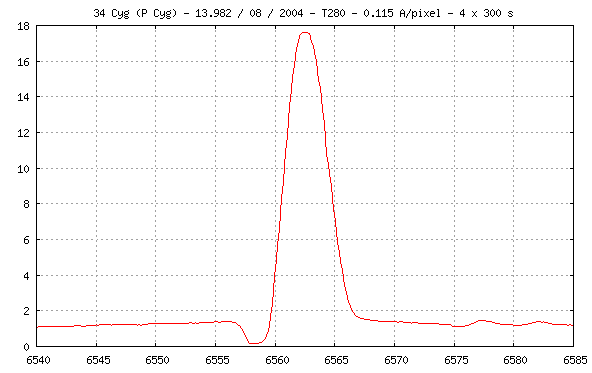
\includegraphics[scale=.40]{figures/34cygni.png}
\caption{The normalised spectrum of 34 Cygni around H$\upalpha$.}
\end{figure}

It is hypothesised that distinct physical processes within these stars generate the respective line profiles \cite{hou2016catalog}. Beals was the first to demonstrate that P Cygni and Inverse P Cygni line profiles can be explained by the interaction between the stellar disk of a hot, massive young star and the expanding or contracting shell of gas surrounding the star \cite{1953PDAO....9....1B}. 

\begin{figure}[!htb]
\centering
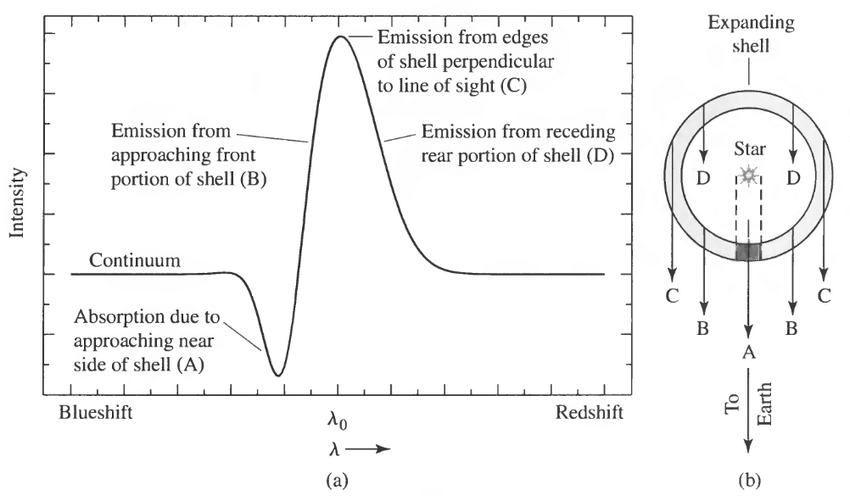
\includegraphics[scale=.40]{figures/expandingpcygni.png}
\caption{Cartoon depicting the physical mechanism by which a P Cygni line profile is generated. Reproduced from Kasai (2013)\cite{kasai2013type}.}
\end{figure}

The P Cygni line profile observed is thus a result of an expanding shell of gas around the main disk of the young hot star. The segment of this shell along the ling of sight contributes to the generation of the absorption line in the spectrum. An average or normal main sequence star will only show a significantly deep absorption line/trough near H$\upalpha$. However, note that in the case of P Cygni, the regions B, C and D of the shell contribute to an emission line. This emission line can occur near H$\upalpha$. As we move from B to C, the intensity of the emission line increases until we reach the edge of the shell. Beyond this point the shell is receding with respect to the line of sight and the intensity of the emission line decreases. It is believed that the opposite process occurs in the case of an inverse P Cygni star. In this case, the shell of gas is contracting and this inflow is responsible for the blue shifted emission line, often to the left of H$\upalpha$. A full discussion of other classes of emission-line stars such as those presented in figure 1.3 and the physics that generate the observed line profiles is beyond the scope of this thesis. However, this work will present suitable classes of such candidates in the GALAH survey where relevant.

\begin{figure}[!htb]
\centering
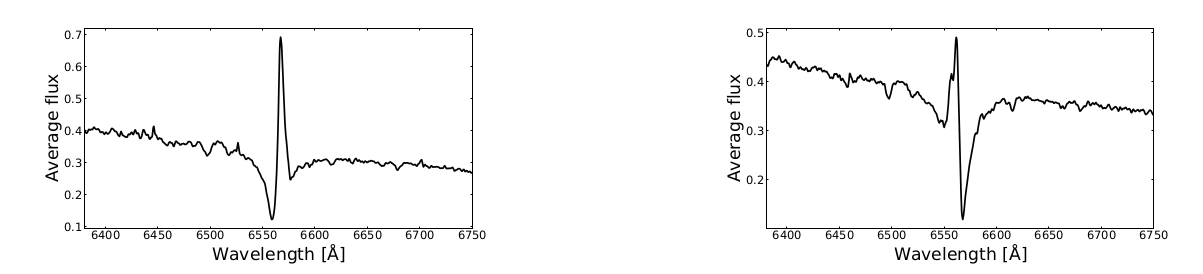
\includegraphics[scale=.48]{figures/p cygni and inverse p cygni.png}
\caption{Four classes of emission-line spectra identified in the Gaia-ESO Survey. Reproduced from Traven et al.\cite{traven2015gaia}}
\end{figure}

\section{A Brief History of Classification}
One of the first modern attempts at identification and classification emission-line stars and in particular P Cygni stars, was by Beals in 1953 \cite{1953PDAO....9....1B}. This work compiled Northern Hemisphere observations of emission-line stars into a comprehensive catalog. This catalog was compiled by examining spectra visually, during a period of observation between the years 1928 and 1946. The catalog was then used to generate hypotheses of how P Cygni stars may exchange material with their surroundings via accretions, inflows and outflows. The morphological properties of the spectra were subsequently used to calculate the wind velocities of inflows and outflows. Manual classification and visual observation of spectral plots was suitable in this context since the volume of data was not significant. However such an approach would not be suitable in the modern era due to the reasons outlined above.

\begin{figure}[!htb]
\centering
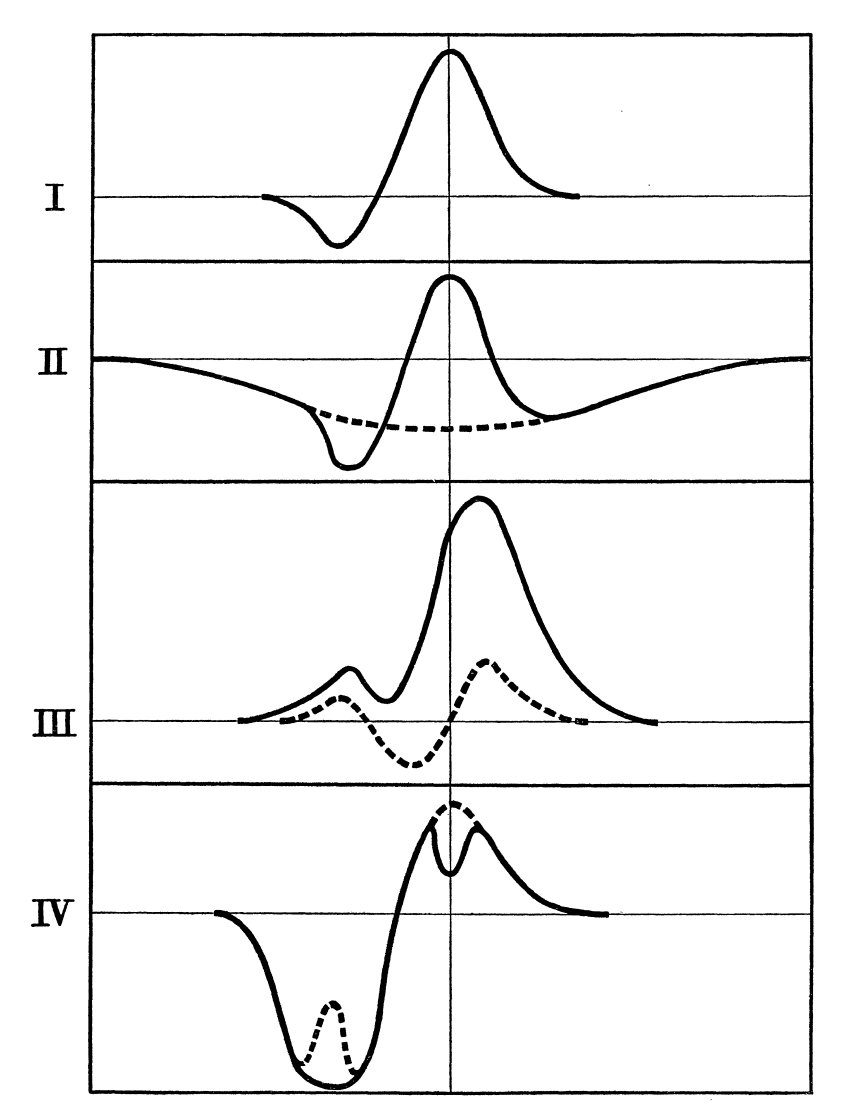
\includegraphics[scale=.30]{figures/beals class 1.png}
\caption{The primary morphological classes of emission-line spectra proposed by Beals (1953) \cite{1953PDAO....9....1B}.}
\end{figure}

The work also presents an early attempt at classification of emission-line stars based on their morphologies. The classification provided by Beals is simpler than modern schemes \cite{reipurth1996hupalpha}. In addition to the primary classes, Beals proposed a set of non-typical classes which were also considered to be P Cygni spectra. This work does not consider these non-typical classes to be P Cygni spectra but rather consider them to be other subgroups of emission line spectra. This approach is congruent with modern research \cite{vcotar2021galah}\cite{zhang2021catalog}\cite{reipurth1996hupalpha} which promote constraints on the classification of P Cygni and inverse P Cygni morphologies. 

Subsequent work such as Reipurth et al. \cite{reipurth1996hupalpha} also relied on manual human classification of emission-line stars based on the morphological properties of the spectra. This was a common trend towards the end of the 20th century as the volume of data was not sufficiently significant to warrant the use of data driven and machine learning based classification routines. However with the advent of large scale spectroscopic surveys and significant advances in computational resources and machine learning techniques, the stage was finally set for data driven classification of machine learning techniques such as the use of t-SNE in 2017 \cite{traven2017galah} and the use of a neural network as an anomaly detector in 2021\cite{vcotar2021galah}. A more detailed review of these efforts, their strengths and weaknesses are presented in subsequent chapters, notably in Chapter 3.

\begin{figure}[!htb]
\centering
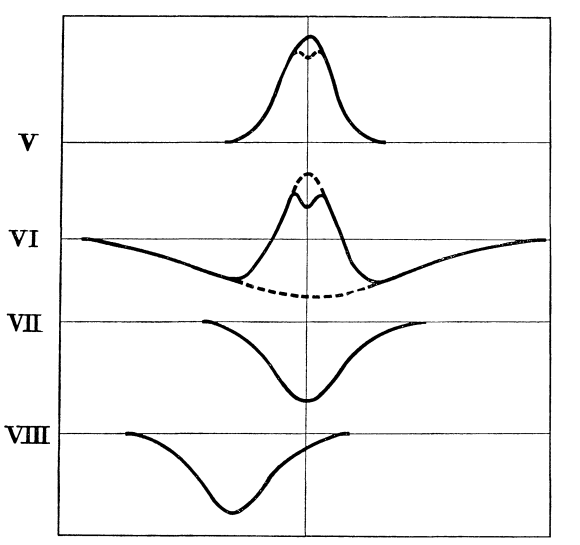
\includegraphics[scale=.50]{figures/beals class 2.png}
\caption{Secondary morphological classes proposed by Beals.}
\end{figure}


